\documentclass[reqno]{article}
\usepackage{../format-doc}
\usepackage{tikz-cd}
\usepackage{subcaption}

\DeclareRobustCommand{\divby}{%
  \mathrel{\vbox{\baselineskip.65ex\lineskiplimit0pt\hbox{.}\hbox{.}\hbox{.}}}%
}

\begin{document}
	\title{Hydrodynamics of liquid crystals using a Maier-Saupe free energy}
	\author{Lucas Myers}
	\maketitle

  \section{Introduction}
  Nematic liquid crystals constitute an interesting phase between crystals and
  typical fluids because they exhibit orientational order, but lack
  translational order.
  Thus their molecules tend to orient themselves along the same axis for thermodynamic
  reasons, but their evolution is also mediated by flows throughout the system.
  Further, topological defects can arise when molecular orientations wrap around
  points or lines in nontrivial ways.
  It is a considerable challenge to properly couple both the thermodynamic
  effects of alignment with the hydrodynamic flow effects, especially when the
  topological nature of defects makes it necessary to introduce a tensor-valued
  order parameter to keep track of the liquid crystal state.
  Here we describe one of the previously-proposed hydrodynamic models, and
  adjust the bulk free energy so that the model can describe anisotropic
  elasticity -- that is, a system in which different types of molecular
  distortions are preferred differently by the system.

  To begin, we give an introduction to liquid crystal theory, first in the
  equilibrium case and then in the non-equilibrium case describing both the
  typical Landau-de Gennes free energy, and then the somewhat lesser-used
  Maier-Saupe mean-field free energy.
  After this we introduce the hydrodynamic model, and subsequently show the
  computational scheme which is used to solve the model.
  To establish the efficacy of our code, we compare configurations prepared by
  our computational scheme to other, previously-established results.
  Finally, we indicate some of the systems and phenomena which we hope to
  investigate with our model.
  
	\section{Equilibrium liquid crystal theory}
	\subsection{The $Q$-tensor}
  The systems that we will be concerned with display a nematic liquid crystal phase.
  The phrase ``liquid crystal'' indicates that the molecules lack positional
  order like a liquid, but they have strong orientational order like a crystal.
  Put another way, the molecules are able to move around one another with
  relative ease, but they tend to align along some preferred direction.
  To display this kind of aligning behavior, the molecules in question must be
  anisotropic in some way.
  In Fig. \ref{fig:cholesteryl-benzoate}, the molecule is completely anisotropic and so we may
  assign a vector roughly along its longest axis, and pointing in some
  particular direction (here we choose towards the benzene rings, but we could
  have just as easily chosen towards the tail).
  \begin{figure}[h] 
    \centering
    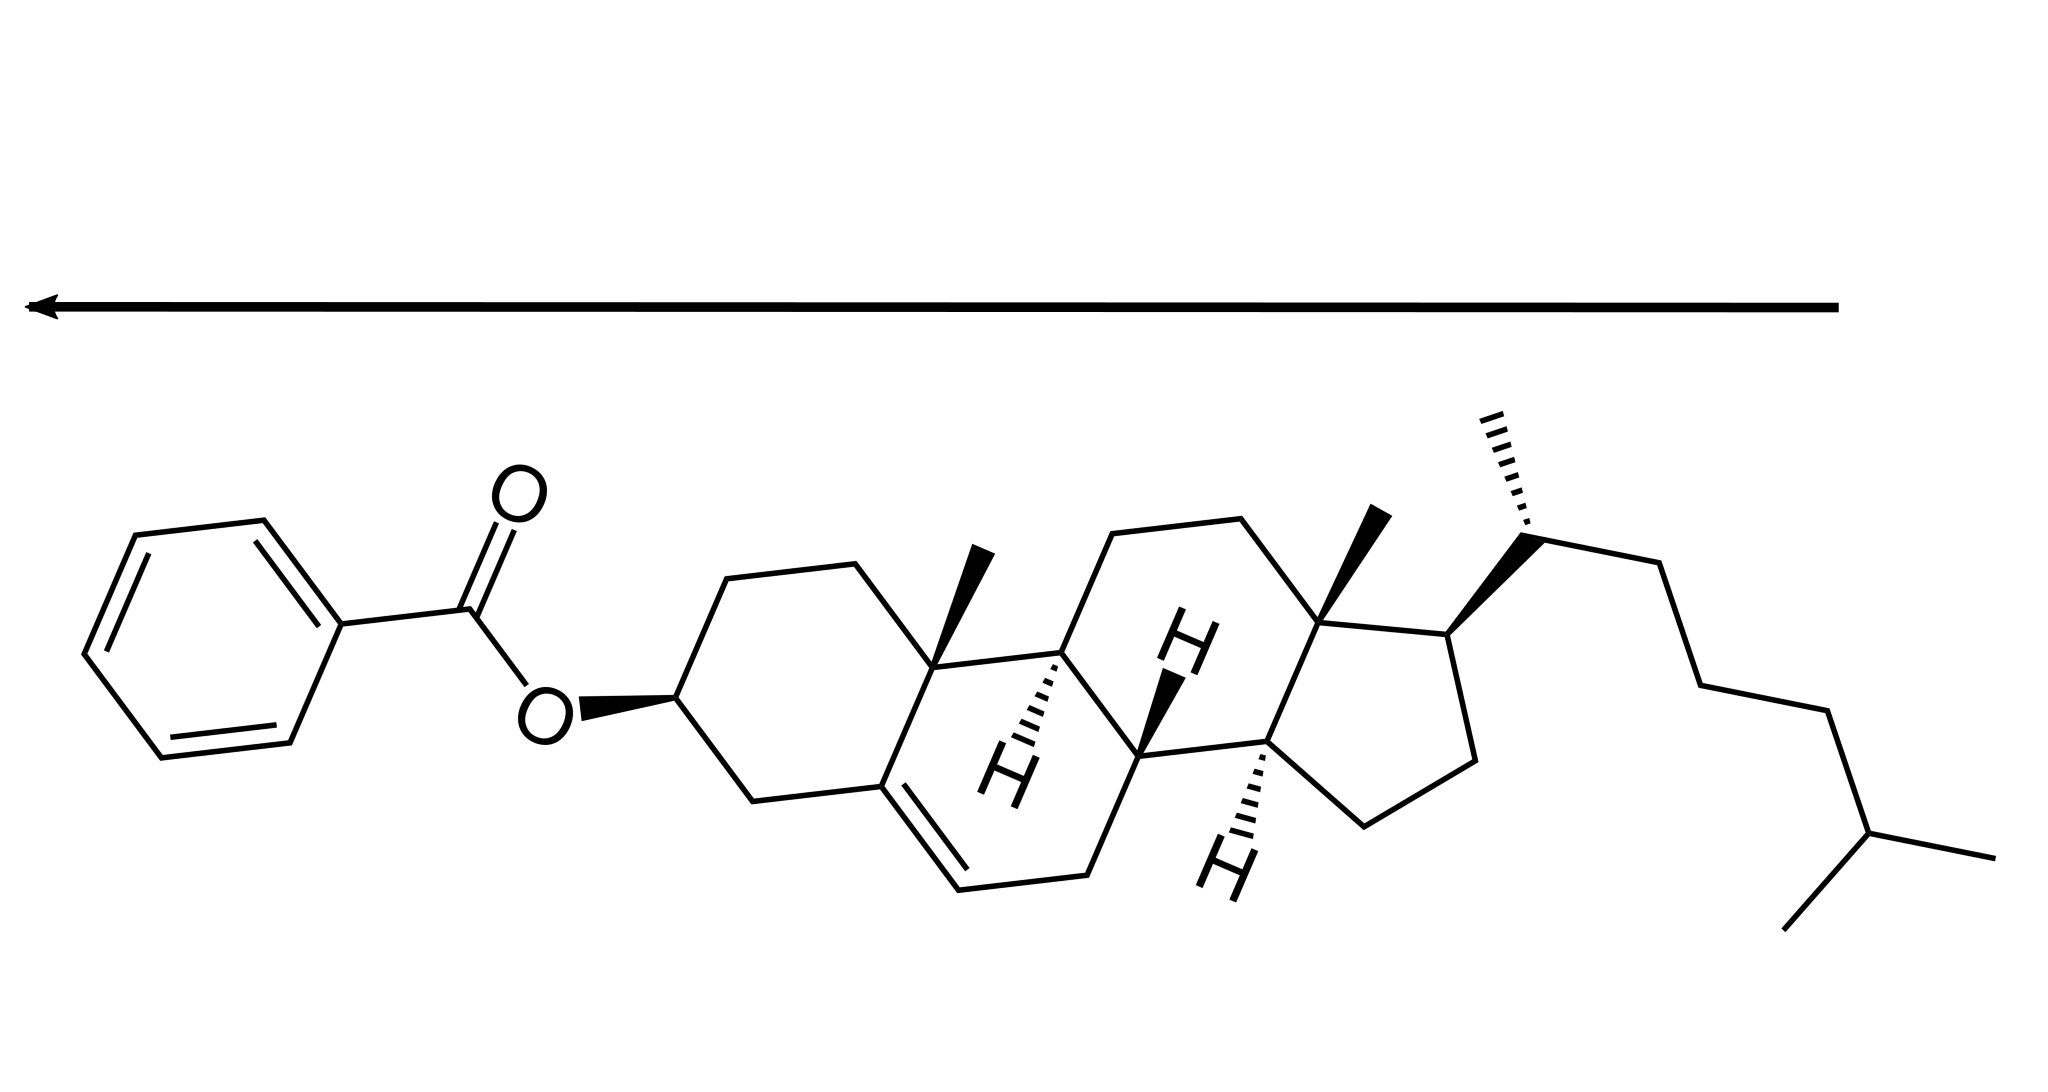
\includegraphics[width=0.6\textwidth]{figures/Cholesteryl_benzoate.png}
    \caption{A cholesteryl benzoate molecule, along with an arrow representing
      a unit vector which we use to characterize its orientation. Image from
      ~\cite{cholesteryl-benzoate}}
    \label{fig:cholesteryl-benzoate}
  \end{figure}

  The two phases that we are interested in are the isotropic phase given in
  Fig. \ref{fig:isotropic-cartoon} in which molecules are randomly oriented, and
  the nematic phase given in Fig. \ref{fig:nematic-cartoon} in which the
  molecules are oriented along some particular axis, but not necessarily in the
  same direction.
  \begin{figure}[h] 
    \centering
    \begin{subfigure}{0.4\textwidth}
      \includegraphics[width=\textwidth]{figures/isotropic_cartoon.png}
      \caption{}
      \label{fig:isotropic-cartoon}
    \end{subfigure}
    \hfill
    \begin{subfigure}{0.4\textwidth}
      \includegraphics[width=\textwidth]{figures/nematic_cartoon.png}
      \caption{}
      \label{fig:nematic-cartoon}
    \end{subfigure}
    \caption{Schematic representation of (a) isotropic and (b) nematic alignment
      patterns of molecules. Cartoons from ~\cite{selinger_introduction_2016}}
    \label{fig:alignment-cartoons}
  \end{figure}
  To encode information from the system about the phase, we define a tensorial
  order parameter $Q$ in terms of an average over all of the molecular
  orientations $\mathbf{p}$:
  \begin{equation} \label{eq:Q-def}
    Q = \langle \mathbf{p} \otimes \mathbf{p} \rangle - \tfrac13 I
  \end{equation}
  with $I$ the $3\times 3$ identity matrix.
  Note that this quantity is even in $\mathbf{p}$ because, in the aggregate
  molecules with orientation $\mathbf{p}$ and $-\mathbf{p}$ should be treated
  equally.
  Note also that this quantity is symmetric and traceless, where the latter
  follows because $\mathbf{p}$ is a unit vector.

  To interpret this quantity physically, note that we may diagonalize the tensor into an
  orthonormal eigenbasis with eigenvalues $\{q_1, q_2, -(q_1 + q_2)\}$ and corresponding
  eigenvectors $\{\mathbf{n}, \mathbf{m}, \mathbf{l}\}$:
  \begin{equation}
    \begin{split}
    Q
    &=
    q_1 (\mathbf{n} \otimes \mathbf{n})
    + q_2 (\mathbf{m} \otimes \mathbf{m})
    - (q_1 + q_2) (\mathbf{l} \otimes \mathbf{l}) \\
    &= S (\mathbf{n} \otimes \mathbf{n} - \tfrac13 I)
    + P (\mathbf{m} \otimes \mathbf{m} - \mathbf{l} \otimes \mathbf{l})
    \end{split}
  \end{equation}
  where we have used the fact that $\{\mathbf{n}, \mathbf{m}, \mathbf{l}\}$ form
  an orthonormal basis so that $\mathbf{n} \otimes \mathbf{n} + \mathbf{m}
  \otimes \mathbf{m} + \mathbf{l} \otimes \mathbf{l} = I$ which is basis
  independent, and we have defined $S = \tfrac32 q_1$ and $P = \tfrac12 (q_1 + q_2)$.
  Here $S$ and $P$ are independent parameters, $n$ is defined by a
  polar angle and an azimuthal angle, $m$ is defined by a single angle
  in the plane perpendicular to $n$, and $l$ is completely
  determined.
  Hence, we have five degrees of freedom which matches what we would expect
  from a $3\times 3$ traceless symmetric tensor.
  
  If we consider eq. \eqref{eq:Q-def}, for a set of particles that is uniformly
  distributed in the azimuthal direction about a main axis $n$, then we may
  write each molecule as:
  \begin{equation}
    \mathbf{p}
    =
    \cos\phi \sin\theta \, \mathbf{m}
    + \sin\phi \sin\theta \, \mathbf{l}
    + \cos\theta \, \mathbf{n}
  \end{equation}
  We call these types of systems ``uniaxial'' because the molecules point mainly
  along one axis.
  If we calculate $Q$, we get:
  \begin{equation} \label{eq:uniaxial-Q-decomposition}
      Q
      = 
      \left< \cos^2 \theta - \tfrac13 \right> \mathbf{n} \otimes \mathbf{n}
      - \tfrac12 \left< \cos^2\theta - \tfrac13 \right> \mathbf{m} \otimes \mathbf{m}
      - \tfrac12 \left< \cos^2\theta - \tfrac13 \right> \mathbf{l} \otimes \mathbf{l}\\
  \end{equation}
  where any term with $\cos\phi$ or $\sin\phi$ has gone to zero, and any term
  with $\sin^2\phi$ or $\cos^2\phi$ has gone to $\tfrac12$.
  Now we may simply read off the eigenvalues of $Q$ to find that:
  \begin{equation}
    S
    = \tfrac32 \langle \cos^2 \theta - \tfrac13 \rangle
    = \langle P_2(\cos\theta) \rangle
  \end{equation}
  where $P_2$ is the second Legendre polynomial.
  Hence, if $S = 1$ we have that $\theta = 0$ always which corresponds to
  perfect alignment.
  Otherwise, if $\theta$ is uniformly distributed we have that $S = 0$.
  Thus, $S$ characterizes the degree of alignment and $\mathbf{n}$ -- sometimes called
  the ``director'' -- characterizes the direction of alignment in uniaxial
  nematics.
  Indeed, historically the development of liquid crystal theory has used the
  director and scalar order parameter $S$ to describe the evolution of nematic
  systems ~\cite{ericksen_hydrostatic_1962, ericksen_liquid_1991}.
  
  \subsection{Landau-de Gennes free energy}
  To predict the equilibrium configuration of a liquid crystal system, we must
  first write down a free energy as a function of the order parameter, and then
  find the order parameter value which minimizes this free energy.
  As a first approach, we recount the method elucidated by Landau and applied to
  nematic liquid crystal systems by de-Gennes.
  This is done by first assuming that the free energy is a smooth function, and
  then Taylor expanding in the appropriate order parameter, in this case the
  $Q$-tensor.
  Additionally, we only keep terms which obey the symmetry of the system.
  For us, these are terms which can undergo an arbitrary rotation, given that
  the direction of alignment will correspond to a broken symmetry when the phase
  transitions from the isotropic state to the nematic state.

  Given that we have a tensor-valued order parameter, the terms which are
  unchanged by rotations are all of the possible ways the $Q$-tensor can be
  contracted to get a scalar value.
  In order to see a first-order phase transition from isotropic to nematic
  phases, one must expand up to fourth order in $Q$:
  \begin{equation}
    F(Q)
    =
    \frac12 A (Q:Q)
    + \frac13 B (QQ):Q
    + \frac14 C_1 (Q:Q)^2
    + \frac18 C_2 (QQ):(QQ)
  \end{equation}
  where here juxtaposition means standard matrix multiplication $QQ \to Q_{ik}
  Q_{kj}$, and dots indicate contraction over indices from innermost to
  outermost $Q:Q \to Q_{ij} Q_{ji}$.
  $A, B, C_1$, and $C_2$ are all imperical quantities.
  Note that:
  \begin{equation}
    (Q:Q)^2 = 2(QQ):(QQ)
  \end{equation}
  which can be seen most easily by choosing a basis wherein $Q$ is diagonal
  (both quantities are scalar and are therefore unchanged by rotations), and
  then explicitly calculating the contractions.
  Given this, we can define $C = (C_1 + \tfrac12 C_2)$ to get only three terms in
  our free energy:
  \begin{equation} \label{eq:landau-de-gennes-bulk-energy}
    F(Q)
    =
    \frac12 A(Q:Q)
    + \frac13 B (QQ):Q
    + \frac14 C (Q:Q)^2
  \end{equation}
  For a uniaxial nematic ($P = 0$) the free energy only depends on the scalar
  order parameter $S$, given that it must be insensitive to rotations.
  $A$ is typically taken to be linear in temperature for thermotropic liquid
  crystals $A = a(T - T_0)$ with $T_0$ some reference temperature, and so we plot
  the free energy for several values of $A$ which corresponds to several
  temperatures in \ref{fig:ldg-free-energy}.
  
  \begin{figure}[h]
    \centering
    \begin{subfigure}{0.45\textwidth}
      \includegraphics[width=\textwidth]{figures/LdG_free_energy.png}
      \caption{Landau-de Gennes bulk free energy}
      \label{fig:ldg-free-energy}
    \end{subfigure}
    \hfill
    \begin{subfigure}{0.45\textwidth}
      \includegraphics[width=\textwidth]{figures/MS_free_energy.png}
      \caption{Maier-Saupe bulk free energy}
      \label{fig:ms-free-energy}
    \end{subfigure}
    \caption{Landau-de Gennes and Maier-Saupe bulk free energies as a function
      of the scalar order parameter $S$ for a uniaxial system. For LdG we vary
      the $A$ parameter in terms of $A_{IN}$, and for MS we vary $\alpha / n
      k_BT$ around $3.4049$, both being the value at which the
      isotropic-nematic transition occurs.}
  \end{figure}
  At low temperatures, the global minimum is at $S \neq 0$ so that the system is
  in a nematic state, whereas at high temperatures the global minimum is at $S =
  0$, the isotropic state.
  There is a cross-over at $A = A_{IN}$ at which point we have a coexistence region
  between isotropic and nematic phases.
  Thus, the theory correctly predicts a phase change, supposing that the
  empirical parameters have the correct signs.

  \subsection{Maier-Saupe mean-field energy}
  While the Landau approach works for many systems, and is rather powerful given
  its relative simplicity, we seek a theory which is more grounded in the
  microscopic details of the system.
  This will allow us to write a theory which has far fewer undetermined factors
  such as the $A, B, C$ of Landau-de Gennes, as well as avoid some pitfalls when
  we venture into nonequilibrium thermodynamics in
  \ref{nonequilibrium-dynamics}.
  
  To begin, we write down an average energy corresponding to the nematic system
  which will then help us write down a free energy.
  Rather than trying to enumerate the average energy from pairwise interactions
  between particles, we make a mean-field approximation whereby each molecule
  interacts with an effective potential produced by all other molecules.
  In this way, we can uncouple fluctuations of individual molecules, and thus
  neglect correlations between their orientations.

  To start, we assume that the pair-wise particle energy of the liquid crystal
  molecules is only dependent on relative angle $\gamma$ get:
  \begin{equation} \label{eq:maier-saupe-pairwise}
    U = -J P_2 \cos(\gamma) = -J \left[ \frac32 \cos^2(\gamma) - \frac12 \right]
  \end{equation}
  Here $J > 0$ so that the energy is minimized when $\gamma$ is a multiple of
  $\pi$ (i.e. the particles are aligned or antialigned).
  One may derive this potential in any number of ways, including a quantum
  mechanical calculation of the dipole interactions between particles, an
  excluded volume calculation by treating the particles as cylinders, or by
  taking the pairwise energy as an arbitrary function of orientation and
  expanding in spherical harmonics.

  In any case, we may calculate for particles with orientations $\mathbf{p}$ and
  $\mathbf{q}$ that:
  \begin{equation}
    \langle \cos^2(\gamma) \rangle
    =
    \langle (\mathbf{p}\cdot \mathbf{q}) (\mathbf{p} \cdot \mathbf{q}) \rangle
    =
    \langle (\mathbf{p} \otimes \mathbf{p}) : (\mathbf{q} \otimes \mathbf{q}) \rangle
    \approx
    \langle (\mathbf{p} \otimes \mathbf{p}) \rangle : \langle (\mathbf{q} \otimes \mathbf{q}) \rangle
  \end{equation}
  where in the last line we have used the mean-field theory that each molecule
  only interacts with an effective field from the other molecules, and so
  fluctuations in $\mathbf{p}$ should be independent of fluctuations in
  $\mathbf{q}$.
  Using this along with the definition of $Q$, we may estimate the average
  energy of the entire system by:
  \begin{equation}
    \langle E \rangle
    =
    -\alpha \, Q : Q
  \end{equation}
  with $\alpha = \frac13 N q J$ where $N$ is the number of molecules, and $q$ is
  the number of neighbors that each particle interacts with.

  Now that we have an energy as a function of the order parameter, we must write
  down a free energy.
  This is done in the usual way, using the definition of the free energy in
  terms of the entropy:
  \begin{equation} \label{eq:standard-free-energy}
    F = \langle E \rangle - TS_\text{entropy}
  \end{equation}
  where
  \begin{equation}
    S_\text{entropy}
    =
    -n k_B \int_{S^2} \rho(\mathbf{p}) \log \left( 4 \pi \rho(\mathbf{p})\right) dS (\mathbf{p})
  \end{equation}
  where the probability distribution function $\rho(\mathbf{p})$ describes the probablility
  that a particular molecule be pointing in some direction given by a point $\mathbf{p}$ on
  the unit sphere $S^2$, $n$ is the number density of the molecules, and $dS$ is
  the surface measure of $S^2$.
  Note that, because the interaction energy only depends on the relative angle
  modulo $\pi$, we have that $\rho(\mathbf{p}) = \rho(-\mathbf{p})$.

  To determine $S_\text{entropy}$ as a function of the order parameter $Q$, we first consider
  its definition in terms of the probability distribution:
  \begin{equation} \label{eq:Q-prob}
    Q
    =
    \int_{S^2} \left(\mathbf{p} \otimes \mathbf{p} - \tfrac13 I\right) \rho(\mathbf{p}) dS(\mathbf{p})
  \end{equation}
  Given that there are many potential $\rho(\mathbf{p})$ functions which will produce a
  particular value for $Q$, we seek the one which will maximize $S_\text{entropy}$.
  This may be done via the method of Lagrange multipliers, by first fixing a
  value of $Q$ and then taking \eqref{eq:Q-prob} to be a constraint on $\rho(\mathbf{p})$.
  The resulting Lagrangian is given as:
  \begin{equation} \label{eq:Lagrangian}
    \begin{split}
      \mathcal{L}[\rho]
      &=
      S_\text{entropy} + \Lambda : \left( \int_{S^2} \left(\mathbf{p} \otimes \mathbf{p} - \tfrac13 I\right) \rho(\mathbf{p}) dS(\mathbf{p}) - Q \right) \\
      &=
      \int_{S^2} \rho(\mathbf{p})
      \left( -n k_B \log \left( 4 \pi \rho(\mathbf{p}) \right) + \Lambda : (\mathbf{p} \otimes \mathbf{p} - \tfrac13 I) \right) dS(\mathbf{p}) - \Lambda : Q
    \end{split}
  \end{equation}
  where $\Lambda$ is a tensorial Lagrange multiplier.
  Note that \eqref{eq:Q-prob} actually only defines five constraints, because
  the fixed $Q$ will be tracless and symmetric by definition, and the integral
  around the sphere has a traceless and symmetric integrand regardless of
  $\rho(\mathbf{p})$.
  Hence, if $\rho(\mathbf{p})$ satisfies the five constraints corresponding to the five
  degrees of freedom of $Q$ then it will necessarily satisfy the other
  (redundant) constraints.
  For the sake of finding a unique set of Lagrange multiplier values, we then
  take $\Lambda$ to also be traceless and symmmetric so that only the unique constraint
  equations show up in \eqref{eq:Lagrangian}.
  
  To maximize the Lagrangian, we take the variation, which yields:
  \begin{equation}
    \delta \mathcal{L}
    =
    \int_{S^2} \left(
      -n k_B \log \left( 4 \pi \rho(\mathbf{p}) \right)
      + \Lambda : (\mathbf{p} \otimes \mathbf{p} - \tfrac13 I)
      - n k_B
    \right) \delta \rho \: dS(\mathbf{p})
  \end{equation}
  For the above to be zero for an arbitrary variation $\delta \rho$, we must have
  that the factor in parentheses is zero.
  Solving the expression for $\rho(\mathbf{p})$ yields:
  \begin{equation}
    \rho(\mathbf{p})
    =
    \frac{1}{4\pi}
    \exp \left(
      -\left(\frac{1}{n k_B} \frac13 \Lambda : I + 1\right)
    \right)
    \exp \left(
      \frac{1}{n k_B} \Lambda : (\mathbf{p} \otimes \mathbf{p})
    \right)
  \end{equation}
  We have one further restriction on $\rho(\mathbf{p})$, which is that it integrates to
  one.
  Dividing by its integral around the sphere cancels the factors out front which
  are constant in $\mathbf{p}$.
  Further, we redefine $\Lambda \to n k_B \: \Lambda$, so that the expression
  simplifies to:
  \begin{equation}
    \rho(\mathbf{p})
    =
    \frac{\exp \left( \mathbf{p}^T \Lambda \, \mathbf{p} \right)}{Z[\Lambda]}
  \end{equation}
  with the partition function $Z[\Lambda]$:
  \begin{equation}
    Z[\Lambda] = \int_{S^2} \exp \left( \mathbf{p}^T \Lambda \, \mathbf{p} \right) dS(\mathbf{p})
  \end{equation}
  Note that we have used the identity $\Lambda : (\mathbf{p} \otimes \mathbf{p}) = \mathbf{p}^T
  \Lambda \, \mathbf{p}$ which is a simple computation using Cartesian coordinates.

  Given this, we may find $\Lambda$ implicitly as a function of $Q$ from
  \eqref{eq:Q-prob}:
  \begin{equation} \label{eq:Q-Lambda}
    \begin{split}
      Q
      &=
      \frac{1}{Z} \int_{S^2} \exp(\mathbf{p}^T \Lambda \, \mathbf{p}) \left( \mathbf{p} \otimes \mathbf{p} - \tfrac13 I \right) dS(\mathbf{p}) \\
      &=
      \frac{\partial \log Z}{\partial \Lambda} - \frac13 I
    \end{split}
  \end{equation}
  where we have integrated the second term using the definition of $Z$.
  Additionally, we have an explicit expression for $S_\text{entropy}$ in terms
  of the Lagrange multiplier $\Lambda$:
  \begin{equation}
    \begin{split}
      S_\text{entropy}
      &=
      -n k_B \,
      \frac{1}{Z}
      \int_{S^2}
      \exp(\mathbf{p}^T \Lambda \, \mathbf{p}) \left( \log 4 \pi + \mathbf{p}^T \Lambda \, \mathbf{p} - \log Z \right) dS(\mathbf{p}) \\
      &=
      -n k_B \left(
        \log 4 \pi - \log Z + \Lambda : \left( Q + \tfrac13 I \right)
      \right)
    \end{split}
  \end{equation}
  where we have again used the definition of $Z$ and expression for $Q$ to
  compute the integrals.

  Supposing that we may invert \eqref{eq:Q-Lambda} -- we will do this
  numerically in section \ref{numerical-scheme} -- we have an expression for the
  free energy in terms of $Q$.
  Given that the free energy is a scalar, it is rotationally invariant and so
  for a uniaxial system ($P = 0$) the free energy should only be a function of
  the scalar order parameter $S$.
  We plot the free energy below for three different temperatures in \ref{fig:ms-free-energy}
  For high temperatures, we see there is one minimum at $S = 0$ which
  corresponds to an isotropic state.
  At lower temperatures, there is one minimum at $S > 0$ which corresponds to a
  (partially) nematically ordered state.
  At some critical temperature $T_C$, we see that there are two minima, one at
  $S = 0$ and one at $S > 0$ at which point the isotropic and nematic phases can
  coexist.
  Again, the theory correctly predicts a phase transition, but has far fewer
  undetermined parameters, and will also be able to handle a wider variety of systems.

  \section{Nonequilibrium dynamics} \label{nonequilibrium-dynamics}

  \subsection{Maier-Saupe field theory}
  To extend the model to the case of nonequilibrium dynamics, we use the field
  theory presented in (cite Majumdar) wherein the order parameter is assumed to
  be in local equilibrium over a small volume at every point in space.
  In this case, $\Lambda$ also becomes a function of position, and the free
  energy becomes a free energy density which must be integrated over space:
  \begin{equation}
    f_b
    =
    -\alpha Q : Q
    - n k_B T \left(\log 4 \pi - \log Z + \Lambda : \left(Q + \tfrac13 I \right) \right)
  \end{equation}
  Here we have labeled the free energy density to indicate that it corresponds
  to a \textit{bulk} free energy.
  
  To account for spatial variation in the order parameter field over the domain,
  we must introduce elastic terms to the free energy density.
  The standard way of going about this for a uniaxial nematic with a fixed
  scalar order parameter $S$ is to write down all possible gradients in the
  director field up to second order which are invariant under spatial rotations
  and sign change of the director.
  The result consists of four terms (supposing molecules are achiral), called
  the Frank elastic terms.
  In general, these have four different associated elastic constants $K_1, K_2,
  K_3, K_4$ which correspond to splay, twist, bend, and saddle-splay distortions of the
  director field respectively -- see Fig. \ref{fig:deformation-cartoon} for a visualization of the first
  three of these modes.
  
  \begin{figure}[h]
    \centering
    \begin{subfigure}{0.45\textwidth}
      \includegraphics[width=\textwidth]{figures/splay_cartoon.png}
      \caption{}
      \label{fig:splay-cartoon}
    \end{subfigure}
    \hfill
    \begin{subfigure}{0.45\textwidth}
      \includegraphics[width=\textwidth]{figures/twist_cartoon.png}
      \caption{}
      \label{fig:twist-cartoon}
    \end{subfigure}
    \hfill
    \begin{subfigure}{0.45\textwidth}
      \includegraphics[width=\textwidth]{figures/bend_cartoon.png}
      \caption{}
      \label{fig:bend-cartoon}
    \end{subfigure}
    \caption{A cartoon of different possible gradients that the director can
      undergo. In (a) splay, the gradient direction points perpendicular to the
      main director component, but parallel to the varying component. In (b)
      twist, the gradient direction points perpendicular to the main director
      component, and perpendicular to the varying component. In (c) bend, the
      gradient direction is parallel to the main director component and
      perpendicular to the varying component. This figure is taken from
      ~\cite{selinger_introduction_2016}.}
    \label{fig:deformation-cartoon}
  \end{figure}
  It happens that $K_4$ is a divergence of a field, and so can be reduced to a
  surface integral by the divergence theorem.
  For now we fix the configuration at the boundaries (Dirichlet conditions) and
  so the saddle-splay term is inconsequential for our model.

  To extend this these terms to a tensor theory, we consider the possible
  invariants which involve gradients of the $Q$-tensor, and then use those which
  reduce to the Frank elastic terms in the case of a uniaxial, constant
  scalar-order nematic.
  These are as follows:
  \begin{equation} \label{eq:elastic-free-energy}
    f_e (\nabla Q)
    = L_1 \left| \nabla Q \right|^2
    + L_2 \left| \nabla \cdot Q \right|^2
    + L_3 \nabla Q  \divby \left[ \left( Q \cdot \nabla \right) Q \right]
  \end{equation}
  In index notation this reads:
  \begin{equation}
    f_e (Q, \nabla Q)
    =
    L_1 \left( \partial_k Q_{ij} \right)^2
    + L_2 \left( \partial_j Q_{ij} \right)^2
    + L_3 Q_{lk} \left( \partial_{l} Q_{ij} \right) \left( \partial_k Q_{ij} \right)
  \end{equation}
  These elastic constants may be written in terms of the Frank elastic constants
  and the constant scalar order parameter.
  Note that, given the added freedom of a tensorial order parameter to capture
  nonuniform order and biaxiality, there are much more complicated theories that
  one may write down in principle.
  
  For our simplified system, the total free energy is then given by an integral
  of the free energy densities over the domain:
  \begin{equation}
    F
    = \int_\Omega f_b(Q) + f_e(Q, \nabla Q) dV
    = \int_\Omega f(Q, \nabla Q) dV
  \end{equation}
  Then, for a purely thermodynamically-driven system, the time evolution
  of the order parameter can be found
  by taking the negative variation of the free energy with respect to the order
  parameter:
  \begin{equation}
    \begin{split}
    -\delta F
    &= -\int_\Omega \left( \frac{\partial f}{\partial Q} \delta Q
      + \frac{\partial f}{\partial (\nabla Q)} \delta (\nabla Q) \right) dV \\
    &= -\int_\Omega \left(
      \frac{\partial f}{\partial Q}
      - \nabla \cdot \frac{\partial f}{\partial (\nabla Q)}
    \right) \delta Q \, dV
    \end{split}
  \end{equation}
  The time evolution of the order parameter field is then the traceless,
  symmetric part of the factor in parentheses:
  \begin{equation}
    \frac{\partial Q}{\partial t}
    =
    -\frac{\partial f}{\partial Q}
    + \nabla \cdot \frac{\partial f}{\partial (\nabla Q)}
  \end{equation}
  In order so maintain the traceless and symmetric character of $Q$, we must
  introduce a Lagrange multiplier scheme which adds the following constraints to
  the free energy:
  \begin{equation}
    f_l (Q) = \lambda_0 Q : I + \lambda \cdot \left( \varepsilon : Q \right)
  \end{equation}
  where $\lambda_0$ is a scalar Lagrange multiplier enforcing $Q$ be traceless,
  $\lambda$ is a vector Lagrange multiplier enforcing $Q$ be symmetric, and
  $\varepsilon$ is the Levi-Civita tensor.
  
  An explicit calculation of the time evolution yields:
  \begin{equation} \label{eq:Q-time-evolution}
    \frac{\partial Q}{\partial t}
    =
    \begin{multlined}[t]
      2 \alpha Q - n k_B T \Lambda + 2 L_1 \nabla^2 Q \\
      + L_2 \left(
        \nabla \left( \nabla \cdot Q \right)
        + \left[ \nabla \left( \nabla \cdot Q \right) \right]^T
        - \tfrac23 \left( \nabla \cdot \left( \nabla \cdot Q \right) \right) I
      \right) \\
      + L_3 \left(
        2 \nabla \cdot \left( Q \cdot \nabla Q \right)
        - \left( \nabla Q \right) : \left( \nabla Q \right)^T
        + \tfrac13 \left| \nabla Q \right|^2 I
      \right)
    \end{multlined}
  \end{equation}
  This is the purely thermodynamic time-evolution equation for the order
  parameter $Q$.
  
  \subsection{Topological defects}
  Given that the nematic state can spatially vary, the director
  -- the main axis of molecular orientation -- is a function of position.
  Supposing a fixed $S$ value, and letting $\mathbf{n}$ be undefined at certain
  points, there can be places where $\mathbf{n}$ wraps around points in
  non-trivial ways as in Fig. \ref{fig:defect-cartoons}.
  These structures can be characterized by the number of rotations that the
  director makes along a path around the undefined point.
  That is, for a two-dimensional configuration the director can be characterized
  by an angle $\theta$ that is made with the $x$-axis so that we may define a
  so-called ``topological charge'' $q$ by:
  \begin{equation}
    \frac{1}{2\pi} \oint_\gamma d \theta = q
  \end{equation}
  where $\gamma$ is some closed loop around the defect.

  These are dubbed ``topological'' because $\theta \circ \gamma$ defines a
  mapping from $[0, 1]$ into $\mathbb{RP}^1$ (in two dimensions) which may be identified in a purely
  topological manner with an element of the fundamental group of $\mathbb{RP}^1$
  ~\cite{mermin_topological_1979}.
  Note that the appropriate space for the director is $\mathbb{RP}^1$ because
  we identify $\mathbf{n}$ and $-\mathbf{n}$ in the same way that
  $\mathbb{RP}^1$ is created by identifying antipodal points of $S^1$.
  Additionally, under the isotropic elasticity approximation (see section
  \ref{anisotropic-elasticity}) the topological defects feel an effective
  two-dimensional Coulombic force \cite{selinger_introduction_2016}.
  It is an active area of research to understand the dynamics of defects under
  more general conditions.
  
  \begin{figure}[h]
    \centering
    \begin{subfigure}{0.3\textwidth}
      \includegraphics[width=\textwidth]{figures/plus_half_defect_cartoon.png}
      \caption{$+1/2$ defect}
      \label{fig:plus-half-defect-cartoon}
    \end{subfigure}
    \hfill
    \begin{subfigure}{0.3\textwidth}
      \includegraphics[width=\textwidth]{figures/minus_half_defect_cartoon.png}
      \caption{$-1/2$ defect}
      \label{fig:minus-half-defect-cartoon}
    \end{subfigure}
    \hfill
    \begin{subfigure}{0.3\textwidth}
      \includegraphics[width=\textwidth]{figures/plus_one_defect_cartoon.png}
      \caption{$+1$ defect}
      \label{fig:plus-one-defect-cartoon}
    \end{subfigure}
    \caption{Schematics of topological defects of various charges. Figure from ~\cite{foffano_dynamics_2014}}
    \label{fig:defect-cartoons}
  \end{figure}

  \subsection{Landau-de Gennes and anisotropic elasticity} \label{anisotropic-elasticity}
  A typical approximation that is used when modeling nematic liquid crystals is
  that elasticity is isotropic: that is, each of the deformation modes shown in
  Fig. \ref{fig:deformation-cartoon} are penalized by the same amount in the
  free energy.
  More concretely, $K_1 = K_2 = K_3 = K_4$ which translates, in the tensorial
  picture, to $L_2 = L_3 = 0$.
  However, this is is not always a valid approximation.
  For example, in an actin-based nematic liquid crystal system, it has been shown that the
  ratio of bend to splay constants $K_3 / K_2$ can be varied from about 0.5 to 2
  by varying the filament length, which drastically changes the defect shape
  ~\cite{zhang_interplay_2018-1}.
  This poses a problem, because for a fourth order Landau-de Gennes bulk free
  energy as given in \ref{eq:landau-de-gennes-bulk-energy}, and an elastic free
  energy as given by \ref{eq:elastic-free-energy} with $L_3 \neq 0$, one is able
  to make the free energy arbitrarily large and negative.
  Hence, there is no global minimizer of the free energy functional, and so the
  evolution of such systems is liable to blow up.

  To elucidate this, we do a short calculation on a simple system.
  Consider a nonequilibrium $Q$-configuration given by:
  \begin{equation}
    Q
    =
    \left( S_0 + \epsilon \sin(kx) \right)
    \text{diag}(q_1, q_2, q_3)
  \end{equation}
  Here the director points in a fixed direction along the $x$-, $y$-, or
  $z$-axis dictated by eigenvalues $q_1, q_2,
  q_3$, and varies periodically in the scalar order parameter according to $S_0, \epsilon$,
  and $k$.
  Calculating the bulk free energy density yields:
  \begin{equation}\label{eq:oscillating-bulk-energy}
    f_b(Q)
    =
    \left(S_{0} + \epsilon \sin{\left(k x \right)}\right)^{2}
    \bigl[
    \begin{multlined}[t]
      \tfrac{A}{2} \left(q_{1}^{2} + q_{2}^{2} + q_{3}^{2}\right) \\
      + \tfrac{B}{3} \left(S_{0} + \epsilon \sin{\left(k x \right)}\right) \left(q_{1}^{3} + q_{2}^{3} + q_{3}^{3}\right) \\
      + \tfrac{C}{4} \left(S_{0} + \epsilon \sin{\left(k x \right)}\right)^{2} \left(q_{1}^{2} + q_{2}^{2} + q_{3}^{2}\right)^{2}
      \bigr]
    \end{multlined}
  \end{equation}
  while the elastic free energy density yields:
  \begin{equation} \label{eq:oscillating-elastic-energy}
    f_e(Q, \nabla Q)
    =
    \begin{multlined}[t]
      \bigl[
      L_{1}
      + L_{3} q_{1} \left(S_{0} + \epsilon \sin{\left(k x \right)}\right)
      \bigr]
      \epsilon^{2} k^{2}
      \left(q_{1}^{2} + q_{2}^{2} + q_{3}^{2}\right)
      \cos^{2}{\left(k x \right)}
    \end{multlined}
  \end{equation}
  Clearly $k$ does not control the amplitude in
  \ref{eq:oscillating-bulk-energy}, and will thus not affect the total bulk free
  energy of a configuration, supposing the free energy density is integrated
  over some integer number of oscillations.
  However, from \ref{eq:oscillating-elastic-energy} the total elastic free
  energy is quadratic in $k$.
  Hence, so long as we have that:
  \begin{equation}
    L_3 q_1(S_0 + \epsilon \sin(kx)) < -L_1
  \end{equation}
  on a majority of the domain, then $k$ can increase without bound to give a
  total free energy that is arbitrarily negative.
  This can be accomplished by setting the director along the $y$-axis so that
  $q_1 < 0$, and setting $S_0$ large enough so that the inequality holds.
  This is simulated via the finite element method in
  ~\cite{schimming_numerical_2021}, and it is found that the configuration
  quickly blows up.

  Indeed, a more general result is proved in ~\cite{ball_nematic_2010} which
  shows that for a fourth-order Landau-de Gennes free energy and $L_3 \neq 0$, a system with
  arbitrary Dirichlet boundary conditions can be made to have arbitrarily
  negative free energy.
  This is not the case with the Maier-Saupe free energy.
  With this theory, the Lagrange multiplier values $\Lambda$ diverges to
  infinity as any of the eigenvalues of $Q$ approach the physically allowed
  limits.
  Hence, $S_0$ is limited by these bounds and so, under appropriate conditions
  on the elastic constants, one can show that there is a unique minimizer of the
  Maier-Saupe free energy ~\cite{schimming_numerical_2021}.
  For this reason, the theory is able to simulate elastic anisotropy, while the
  standard Landau-de Gennes theory is not.


  \section{Hydrodynamics}
  The derivation of the time evolution of the system in the preceding section
  assumed a system driven purely by thermodynamics.
  That is, no transfer of mass or corresponding hydrodynamic flow, only transfer of energy and entropy.
  This is insufficient for many cases, however, as one might imagine flows
  having a non-negligible effect on molecular alignment
  ~\cite{svensek_hydrodynamics_2002, toth_hydrodynamics_2002}.
  That said, there is yet to be a hydrodynamic theory for the $Q$-tensor model
  which is generally accepted by the community.
  By using general conservation laws of fluid mechanics applied to the director
  formulation of nematic liquid crystal theory, Ericksen and Leslie were able to
  derive hydrodynamic equations of a uniaxial nematic liquid crystal system with
  constant scalar order ~\cite{ericksen_hydrostatic_1962, Leslie1968}.
  However, it happens that for a more general tensorial theory one needs
  additional contitutive relations in order to produce governing equations.

  There have been several attempts at this, including by Beris and Edwards
  through use of their ``dissipation bracket'', by Qian and Sheng through
  methods similar to Ericksen and Leslie but with additional contitutive
  equations, and by Sonnet and Virga through use of a generalized Rayleigh
  dissipation factor ~\cite{Beris1994, qian_generalized_1998, sonnet_dissipative_2012}.
  All of these models are still poorly characterized and so to follow
  ~\cite{svensek_hydrodynamics_2002} we choose the Qian and Sheng
  formulation.
  They, however, use a Landau-de Gennes expression for the bulk portion of their
  free energy while we use the Maier-Saupe expression presented above.

  In what follows, we merely quote the hydrodynamic equations and explain
  several simplifying assumptions that we make upon a first pass.
  We begin with the equation of motion for the $Q$-tensor:
  \begin{equation} \label{eq:generalized-force-balance}
    J \ddot{Q} = h + h'
  \end{equation}
  Here $J$ is the moment of inertia density (which we will take to be
  negligible), $h$ is the generalized force from thermodynamics and $h'$ is the
  viscous generalized force.
  The generalized force $h$ is given as in section
  \ref{nonequilibrium-dynamics} as:
  \begin{equation}
    h
    =
    -\frac{\partial f}{\partial Q}
    + \nabla \cdot \frac{\partial f}{\partial (\nabla Q)}
    - \lambda_0 Q : I
    - \lambda \cdot \left( \varepsilon : Q \right)
  \end{equation}
  Here we have separated out the Lagrange multipliers $\lambda_0$ and $\lambda$
  once again to constrain $\partial Q/\partial t$ to be symmetric and traceless
  no matter which hydrodynamic terms arise.
  $\lambda_0$ is a scalar, $I$ is the $3\times 3$ identity matrix, $\lambda$ is
  a vector, and $\varepsilon$ is the Levi-Civita symbol.
  The viscous generalized force is given by:
  \begin{equation} \label{eq:viscous-force}
    -h'
    =
    \tfrac12 \mu_2 A
    + \mu_1 N
  \end{equation}
  where $A = \tfrac12 \left( \nabla v + \left( \nabla v \right)^T \right)$ is
  the symmetric part of the velocity gradient tensor, and $N = dQ / dt + (WQ -
  QW)$ is the corotational derivative, representing the time rate of change of
  $Q$ is a frame that rotates with the fluid element.
  Here $d/dt = \partial / \partial t + \nabla \cdot v$ is the material
  derivative, and $W = \tfrac12 \left( \nabla v - \left( \nabla v \right)^T
  \right)$ is the antisymmetric part of the velocity gradient tensor.
  To find an expression for the time evolution of $Q$ we use
  \eqref{eq:viscous-force} and \eqref{eq:generalized-force-balance} to
  solve for $N$:
  \begin{equation} \label{eq:N}
    N = \frac{1}{\mu_1} h - \frac12 \frac{\mu_2}{\mu_1} A
  \end{equation}
  Here we have assumed $J$ to be negligible so that $J\ddot{Q} \approx 0$ in
  \eqref{eq:generalized-force-balance}.
  The definition of $N$ then yields:
  \begin{equation} \label{eq:Q-equation}
    \frac{d Q}{dt}
    =
    \frac{1}{\mu_1} h
    + \left[ Q, W \right]
    - \frac12 \frac{\mu_2}{\mu_1} A
  \end{equation}
  with $\left[ Q, W \right] = QW - WQ$ the commutator.

  The generalized Navier-Stokes equation is given by:
  \begin{equation}
    \rho \frac{dv}{dt}
    =
    \nabla \cdot \left(
      -p I
      + \sigma^d
      + \sigma^f
      + \sigma'
    \right)
  \end{equation}
  with $v$ the velocity, $p$ the pressure, $\sigma^d$ the stress tensor from
  distortions in the nematic field,
  $\sigma^f$ the stress tensor from external fields (i.e. electric and
  magnetic), and $\sigma'$ the viscous stress tensor.
  This along with the incompressibility condition $\nabla \cdot v = 0$ defines
  the system.
  We do not consider external fields so that $\sigma^f = 0$ and we suppose that
  the velocity field adapts quickly to the nematic configuration as argued in
  ~\cite{svensek_complex_2002} so that $dv/dt \approx 0$.
  The elastic stress is given in terms of the free energy density as:
  \begin{equation}
    \sigma^d
    =
    - \frac{\partial f}{\partial (\nabla Q)} : \left( \nabla Q \right)^T
  \end{equation}
  The viscous stress tensor is given by:
  \begin{equation} \label{eq:viscous-stress-tensor}
    \sigma'
    =
    \begin{multlined}[t]
      \beta_1 Q \left( Q : A \right)
      + \beta_4 A
      + \beta_5 QA
      + \beta_6 AQ
      + \frac12 \mu_2 N \\
      - \mu_1 QN + \mu_1 NQ
    \end{multlined}
  \end{equation}
  It has been shown that, in configurations of defect annihilation the $\beta_1,
  \beta_5$, and $\beta_6$ terms are negligible, only producing quantitative
  effects ~\cite{svensek_hydrodynamics_2002}.
  Additionally, we choose to neglect the $\mu_1$ terms.
  These do, in fact, produce a qualitative difference in the case of defect
  annihilation, creating an asymmetry in the trajectory of $+1/2$ and $-1/2$
  defects.
  However, for now we seek to linearize the flow equation so that we only have
  to solve a much simpler Stoke's system.

  These simplifications, along with \eqref{eq:N} give the following flow equation:
  \begin{equation}
    0
    =
    \nabla \cdot \left(
      -p I
      + \sigma^d
      + \beta_4 A
      + \frac{\mu_2}{2 \mu_1} h - \frac{\mu_2^2}{4 \mu_1} A
    \right)
  \end{equation}
  Solving for $A$ yields:
  \begin{equation} \label{eq:stokes-equation}
    -2 \nabla \cdot A + \frac{1}{\gamma_1} \nabla p
    =
    \nabla \cdot \left(
      \frac{1}{\gamma_1} \sigma^d
      + \frac{1}{\gamma_2} h
    \right)
  \end{equation}
  with viscosities $\gamma_1$ and $\gamma_2$ given by:
  \begin{equation}
    \gamma_1
    =
    \frac{\beta_4}{2} - \frac{\mu_2^2}{8 \mu_1},
    \:\:\:\:
    \gamma_2
    =
    \frac{\mu_1 \beta_4}{\mu_2} - \frac{\mu_2}{4}
  \end{equation}
  Hence, equations \eqref{eq:Q-equation} and \eqref{eq:stokes-equation} comprise
  our coupled hydrodynamic and thermodynamic system.
  Note that $\sigma^d$ and $h$ only depend on $Q$, so that we have (somewhat
  artificially) decoupled the right-hand side from flow.
  As a final note, we explicitly calculate $\sigma^d$:
  \begin{equation}
    \sigma^d
    =
    - 2 L_1 \nabla Q : \left( \nabla Q \right)^T
    - L_2 \left( \nabla \cdot Q \right) \cdot \left( \nabla Q \right)^T
    - 2 L_3 \left( Q \cdot \left[ \left( \nabla Q \right) : \left( \nabla Q \right)^T \right] \right)^T
  \end{equation}
  
  \section{Numerical scheme} \label{numerical-scheme}
  To solve these equations numerically, we first discretize in time by using a
  semi-implicit method which leverages convexity of several terms to increase
  the convergence rate.
  Given the semi-implicit time-stepping scheme, as well as the nonlinearity of
  the equations, we must use Newton's method to update the time step.
  Spatial discretization is done by introducing a weak form of the equations,
  and then using a finite element method to solve each of the coupled equations.
  In the course of setting up the finite element system, we will have need of
  inverting the Lagrange multiplier $\Lambda$ and we will also need to find the
  Jacobian of that mapping, due to the overall Newton's method imposed on the
  implicit time-stepping scheme.
  This must be done efficiently, as it happens at every quadrature point in the
  finite element mesh several times per time-step.
  We detail each of these steps below.

  \subsection{Nondimensionalization}
  We begin by nondimensionalizing the generalized force $h$, whose explicit
  expression is exactly the right-hand side of \eqref{eq:Q-time-evolution}.
  To do this, we introduce a length-scale $\xi$ and write gradients as
  derivatives with respect to the nondimensional length $\overline{x} = x /
  \xi$.
  Additionally, we may divide by the energy density $n k_B T$:
  \begin{equation}
    \frac{h}{n k_B T}
    =
    \begin{multlined}[t]
      \frac{2 \alpha}{n k_B T}
      - \Lambda
      + \frac{2 L_1}{n k_B T \xi^2} \nabla^2 Q  \\
      + \frac{L_2}{n k_B T \xi^2} \left(
        \nabla \left( \nabla \cdot Q \right)
        + \left[ \nabla \left( \nabla \cdot Q \right) \right]^T
        - \tfrac23 \left( \nabla \cdot \left( \nabla \cdot Q \right) \right) I
      \right) \\
      + \frac{L_3}{n k_B T \xi^2} \left(
        2 \nabla \cdot \left( Q \cdot \nabla Q \right)
        - \left( \nabla Q \right) : \left( \nabla Q \right)^T
        + \tfrac13 \left| \nabla Q \right|^2 I
      \right)
    \end{multlined}
  \end{equation}
  Now we define the following quantities:
  \begin{equation}
    \begin{split}
      \xi = \sqrt{\frac{2 L_1}{n k_B T}}, \:\:\:\:
      \overline{\alpha} = \frac{2 \alpha}{n k_B T}, \:\:\:\:
      \overline{h} = \frac{h}{n k_B T}, \:\:\:\:
      \overline{L_2} = \frac{L_2}{L_1}, \:\:\:\:
      \overline{L_3} = \frac{L_3}{L_1}
    \end{split}
  \end{equation}
  Substituting and dropping the overlines for brevity, this yields:
  \begin{equation}
    h
    =
    \alpha Q
    - \Lambda
    + \nabla^2 Q 
    + L_2 \, E_2 (Q, \nabla Q) 
    + L_3 \, E_3 (Q, \nabla Q)
  \end{equation}
  with anisotropic elastic terms given by:
  \begin{align}
    E_2 (Q, \nabla Q)
    &=
    \tfrac12 \left[
    \nabla \left( \nabla \cdot Q \right)
    + \left[ \nabla \left( \nabla \cdot Q \right) \right]^T
    \right]
    - \tfrac13 \left( \nabla \cdot \left( \nabla \cdot Q \right) \right) I \\
    E_3(Q, \nabla Q)
    &=
    \nabla \cdot \left( Q \cdot \nabla Q \right)
    - \tfrac12 \left( \nabla Q \right) :  \left( \nabla Q \right)^T
    + \tfrac16 \left| \nabla Q \right|^2 I
  \end{align}

  To nondimensionalize \eqref{eq:Q-equation}, we first note that $A$ and $W$
  have dimensions of inverse time, because the characteristic length scale $\xi$
  cancels between the gradient and the velocity.
  Hence, we may introduce a characteristic time $\tau$ as:
  \begin{equation}
    \frac{1}{\tau} \frac{dQ}{d\overline{t}}
    =
    \frac{n k_B T}{\mu_1} \overline{h}
    + \frac{1}{\tau} [Q, \overline{W}]
    - \frac12 \frac{\mu_2}{\mu_1} \frac{1}{\tau} \overline{A}
  \end{equation}
  Given this, we make the following definitions:
  \begin{equation}
    \tau = \frac{\mu_1}{n k_B T}, \:\:\:\:
    \gamma = -\frac12 \frac{\mu_2}{\mu_1}
  \end{equation}
  Note that $\mu_2/\mu_1$ is typically negative so that the so-called
  flow-alignment parameter $\gamma$ is positive.
  Dropping overlines, this gives:
  \begin{equation}
    \frac{dQ}{dt}
    =
    h + [Q, W] + \gamma A
  \end{equation}

  For the Stokes equation, we begin by nondimensionalizing the elastic stress
  tensor.
  Substituting the characteristic length, we end up with:
  \begin{equation}
    \overline{\sigma}^d
    =
    - \nabla Q : \left( \nabla Q \right)^T
    - \tfrac12 \overline{L}_2 \left( \nabla \cdot Q \right) \cdot \left( \nabla Q \right)^T
    - \overline{L}_3 \left( Q \cdot \left[ \left( \nabla Q \right) : \left( \nabla Q \right)^T \right] \right)
  \end{equation}
  with:
  \begin{equation}
    \sigma^d = \overline{\sigma}^d n k_B T
  \end{equation}
  With this, the flow equation reads:
  \begin{equation}
    -2 \frac{1}{\tau \xi} \nabla \cdot A
    + \frac{1}{\gamma_1} \frac{\eta}{\xi} \nabla p
    =
    \frac{1}{\xi} \nabla \cdot \left(
      \frac{1}{\gamma_1} n k_B T \sigma^d
      + \frac{1}{\gamma_2} n k_B T h
    \right)
  \end{equation}
  Here $\eta$ is a dimensional parameter associated with $p$.
  Multiplying through by $\xi \tau$, and then using the definition of $\tau$ we
  find:
  \begin{equation} \label{eq:stokes-nondimensionalized}
    -2 \nabla \cdot A
    + \nabla p
    =
    \nabla \cdot \left(
      \zeta_1 \sigma^d
      + \zeta_2 h
    \right)
  \end{equation}
  where we have taken:
  \begin{equation}
    \eta = \gamma_1 / \tau, \:\:\:\:
    \zeta_1 = \left( \frac12 \frac{\beta_4}{\mu_1} - \frac18 \left( \frac{\mu_2}{\mu_1} \right)^2 \right)^{-1}, \:\:\:\:
    \zeta_2 = \left( \frac{\beta_4}{\mu_2} - \frac14 \frac{\mu_2}{\mu_1} \right)^{-1}
  \end{equation}
  Hence, the remaining parameters in the system are: the interaction parameter
  $\alpha$ which is controlled by the temperature; the anisotropic elasticities
  $L_2$ and $L_3$; the flow-alignment parameter $\gamma$ which controls the
  nematic's tendency to align along the direction of flow; and the two viscosity
  parameters $\zeta_1$ and $\zeta_2$ which control the relative weight with which
  generalized force and elastic stress tensor affect the flow configuration.
  
  \subsection{Discretization of $Q$-tensor equation}
  Given that the $Q$-tensor is tracless and symmetric, we may write it in terms
  of its degrees of freedom as:
  \begin{equation} \label{eq:Q-degrees-of-freedom}
    Q
    =
    \begin{bmatrix}
      Q_1 & Q_2 & Q_3 \\
      Q_2 & Q_4 & Q_5 \\
      Q_3 & Q_5 & -(Q_1 + Q_4)
    \end{bmatrix}
  \end{equation}
  and collect those degrees of freedom into a five-component vector, $q$:
  \begin{equation} \label{eq:Q-vector}
    q
    =
    \begin{bmatrix}
      Q_1 \\
      Q_2 \\
      Q_3 \\
      Q_4 \\
      Q_5
    \end{bmatrix}
  \end{equation}
  There are several other traceless and symmetric quantities which are functions
  of $Q$ (and therefore may be written as vector functions of $q$), but which
  require tensor contraction operations, and can thus not simply be notated as
  vector operations on $q$.
  In an attempt to compartmentalize cumbersome notation, we collect the degrees
  of freedom of these traceless, symmetric tensors into corresponding vectors,
  and write them as functions of the vector $q$ to get:
  \begin{equation}
    \Lambda (Q) \to \lambda(q), \:\:\:\:
    E_2(Q, \nabla Q) \to e_2(q, \nabla q), \:\:\:\:
    E_3(Q, \nabla Q) \to e_3(q, \nabla q), \:\:\:\: 
    [Q, W] \to c(q), \:\:\:\:
    A \to a
  \end{equation}
  These may be calculated explicitly by writing $Q$ as in
  \eqref{eq:Q-degrees-of-freedom}, calculating the tensorial terms, and then
  taking the appropriate entries to construct a vector as in
  \eqref{eq:Q-vector}.
  For the time evolution of $q$, these expressions will be written explicitly in terms of the
  degrees of freedom $Q_i$.

  To discretize in time we first note that in \eqref{eq:standard-free-energy}
  $-TS_\text{entropy}$ is convex while $\langle E \rangle = -\alpha Q:Q$ is
  concave ~\cite{schimming_numerical_2021}.
  The free energy is then a difference between a convex part and a concave part,
  which is referred to as a convex splitting ~\cite{xu_stability_2019}.
  For systems governed by such a free energy, it happens that treating the
  convex part implicitly and the concave part explicitly can make the scheme
  unconditionally energy-stable, and guarantee convergence in Newton's method
  regardless of the initial guess.
  We do that here, also treating the elastic and hydrodynamic terms implicitly.
  \begin{equation}
    \frac{q - q_0}{\delta t}
    + v \cdot \nabla q
    =
    \alpha q_0
    - \lambda(q)
    + \nabla^2 q
    + L_2 \, e_2(q, \nabla q)
    + L_3 \, e_3(q, \nabla q)
    + c(q)
    + \gamma a
  \end{equation}
  where $q$ is the configuration at the current time-step, $q_0$ is the
  configuration at the previous time-step, and $\delta t$ is the step size.
  Given that this is a nonlinear equation which we seek to solve via a finite
  element method, we must use the Newton-Rhapson method to linearize.
  To that end, we define a vector residual:
  \begin{equation} \label{eq:simulation-residual}
    \mathcal{R}(q^n)
    =
    q^n + v \cdot \nabla q^n
    - (1 + \delta t \, \alpha) q_0
    - 
    \delta t \left(
      -\lambda(q^n)
      + \nabla^2 q^n
      + L_2 \, e_2(q^n, \nabla q^n)
      + L_3 \, e_3(q^n, \nabla q^n)
      + c(q^n)
      + \gamma a
    \right)
  \end{equation}
  where $q^n$ is the value of $q$ for the $n$th Newton iteration.
  Then the iterative method reads:
  \begin{equation}
    \begin{split}
      \mathcal{R}'(q^n) \delta q^n &= -\mathcal{R}(q^n) \\
      q^{n + 1} &= q^n + \alpha_0 \delta q^n
    \end{split}
  \end{equation}
  with $\mathcal{R}'$ the Gateaux derivative of the residual, and $\delta q^n$
  the variation of $q$ which must be solved for at each time step.
  $\alpha_0 < 1$ is a step size that can be made smaller for a system for which
  the convergence is more sensitive.
  Explicitly, the Jacobian $\mathcal{R}'$ reads:
  \begin{equation}
    \mathcal{R}' \delta q^n
    =
      \delta q^n
      + v \cdot \nabla \delta q^n
      -\delta t \biggl[
      \begin{multlined}[t]
        - \left. \left( \frac{\partial \lambda}{\partial q} \right) \right|_{q^n} \delta q^n
        + \nabla^2 \delta q^n \\
        + L_2 e_2'(q^n, \nabla q^n) \, \delta q^n
        + L_3 e_3'(q^n, \nabla q^n) \, \delta q^n
        + c'(q^n) \, \delta q^n
      \biggr]
    \end{multlined}
  \end{equation}
  Here $e_2'$ and $e_3'$ are linear operators which depend on the configuration
  at the last Newton iteration, and contain differential operators.
  $c'$ is a matrix whose values only depend on $q^n$.

  We now cast this linear equation in its weak form by taking an inner product
  with an arbitrary (vector) test function $\varphi$:
  \begin{equation}\label{eq:simple-weak-form}
    \langle \varphi, \mathcal{R}' \delta q \rangle
    = -\langle \varphi, \mathcal{R} \rangle
  \end{equation}
  where here we define the inner product as:
  \begin{equation} 
    \langle f, g \rangle
    =
    \int_\Omega f \cdot g
  \end{equation}
  for the domain $\Omega$.
  To recast this as a discrete problem, we dictate that
  \eqref{eq:simple-weak-form} must be satisfied for some finite-dimensional
  subspace of the space of test functions with basis $\phi_i$.
  Further, we represent the solution $\delta q^n$ (approximately) as a linear
  combination of these basis elements:
  \begin{equation} \label{eq:q-finite-approximation}
    \delta q^n = \sum_{i} \delta q^n_i \varphi_i
  \end{equation}
  Using \eqref{eq:q-finite-approximation} with \eqref{eq:simple-weak-form} and integrating
  by parts, yields an equation with the following form:
  \begin{equation}
    A^n_{ij} \delta q^n_j = b^n_i
  \end{equation}
  with
  \begin{equation}
    A^n_{ij}
    =
    \langle \varphi_i, \varphi_j \rangle
    + \langle \varphi_i, v \cdot \nabla \varphi_j \rangle
    - \delta t \biggl[
    \begin{multlined}[t]
      -\left< \varphi_i, \left( \frac{\partial \lambda}{\partial q} \right) \varphi_j \right>
      - \langle \nabla \varphi_i, \nabla \varphi_j \rangle \\
      + L_2 \langle \varphi_i, e_2' \varphi_j \rangle
      + L_3 \langle \varphi_i, e_3' \varphi_j \rangle
      + \langle \varphi_i, c' \varphi_j \rangle
      \biggr]
    \end{multlined}
  \end{equation}
  and
  \begin{equation}
    b_i
    =
    \begin{multlined}[t]
    \langle \varphi_i, q^n \rangle
    + \langle \varphi_i, v \cdot \nabla q^n \rangle
    - (1 + \delta t \, \alpha) \langle \varphi_i, q_0 \rangle \\
    - \delta t \biggl[
      - \langle \varphi_i, \lambda(q^n) \rangle
      - \langle \nabla \varphi_i, \nabla q^n \rangle
      + L_2 \langle \varphi_i, e_2(q^n) \rangle \\
      + L_3 \langle  \varphi_i, e_3(q^n) \rangle
      + \langle \varphi_i, c(q^n) \rangle
      + \gamma \langle \varphi_i, a(v) \rangle
    \biggr]
    \end{multlined}
  \end{equation}
  Here we have, for the isotropic elasticity terms, integrated by parts:
  \begin{equation}
    \langle \varphi_i, \nabla^2 \varphi_j \rangle
    =
    \langle \varphi_i, n \cdot \nabla \varphi_j \rangle_{\partial \Omega}
    +
    \langle \nabla \varphi_i, \nabla \varphi_j \rangle
  \end{equation}
  where $n$ is the unit vector normal to the boundary $\partial \Omega$, and the
  corresponding inner product is integrated over the boundary.
  For now we assume either Dirichlet or zero-valued Neumann conditions.
  In the former case, the test functions $\varphi_i$ come from the space tangent
  to the solution space so that they are zero on the boundary.
  In the latter case, the normal derivative is zero.
  In both cases, the boundary term vanishes.
  For more general boundary-conditions (nonzero Neumann or mixed), we just end
  up with another term on the right-hand side which can be calculated from the
  values of the normal derivative prescribed at the boundary.

  \subsection{Discretization of the Stokes equation}
  Given that the simplified hydrodynamic model gives the flow velocity in the
  form of a typical Stoke's equation, the discretization is somewhat standard.
  We first collect the equations into a single vector equation:
  \begin{equation}
    \begin{pmatrix}
      -2 \nabla \cdot A(v) + \nabla p \\
      - \nabla \cdot v
    \end{pmatrix}
    =
    \begin{pmatrix}
      \nabla \cdot \left( \zeta_1 \sigma^d + \zeta_2 h \right) \\
      0
    \end{pmatrix}
  \end{equation}
  We then dot with a vector set of test equations $\begin{pmatrix} u &q \end{pmatrix}^T$ with
  $u$ in the space of velocity functions, and $q$ in the space of pressure
  functions.
  This yields:
  \begin{equation}
    \langle u, -2 \nabla \cdot A(v) + \nabla p \rangle - \langle q, \nabla \cdot v \rangle
    =
    \langle u, \nabla \cdot \left( \zeta_1 \sigma^d + \zeta_2 h \right) \rangle
  \end{equation}
  Now we may use the divergence theorem to integrate by parts, and also note
  that:
  \begin{equation}
    \begin{split}
      \tfrac12 \left( \nabla u \right) : \left( \nabla v + \left( \nabla v \right)^T \right)
      &= \tfrac12
      \left(\partial_i u_{j} \right) \left( \partial_j v_i + \partial_i v_j \right) \\
      &= \tfrac14 \left[  \left(\partial_i u_{j} \right) \left( \partial_j v_i + \partial_i v_j \right)
        + \left(\partial_j u_{i} \right) \left( \partial_i v_j + \partial_j v_i \right)
      \right] \\
      &= A(u) : A(v)
    \end{split}
  \end{equation}
  where for the second term in the second equality we have relabeled $i \to j$,
  $j \to i$.
  Given this, the weak form of our equation reads:
  \begin{equation}
    2\langle A(u), A(v)  \rangle
    - \langle \nabla \cdot u, p \rangle
    - \langle q, \nabla \cdot v \rangle
    =
    -\langle \nabla u, \zeta_1 \sigma^d + \zeta_2 h \rangle
  \end{equation}
  Here we have chosen no slip boundary conditions so that the boundary terms
  from the weak form go to zero.

  To discretize, we choose a finite element basis $\varphi_i
  = \begin{pmatrix} \varphi_{i, v} &\varphi_{i, p} \end{pmatrix}$ to act
  as our test functions as well as a basis for our solution.
  The equations in the form above constitute a symmetric saddle-point problem,
  as defined in terms of bilinear forms on the spaces of velocity and pressure
  functions.
  It happens that, in order for the solution to the discretized problem to be
  stable (e.g. not contain artifacts such as spurious oscillations), the
  finite-dimensional solution space must satisfy the
  Ladyzhenskaya-Babuska-Brezzi (LBB) condition, which is a constraint on
  $\langle \nabla \cdot u, p \rangle$ restricted to the finite element space ~\cite{boffi_mixed_2013}.
  We omit the details here, but for our purposes it suffices to choose Lagrange (piece-wise polynomial)
  elements so that the pressure part of the solution $\varphi_{i, p}$ is
  represented by elements of degree $d$, and the velocity solution $\varphi_{i, v}$ is
  represented by elements of degree $d + 1$.
  This then becomes a matrix inversion problem with matrix
  \begin{equation}
    A_{ij}
    =
    2 \langle A(\varphi_{i, v}), A(\varphi_{j, v}) \rangle
    - \langle \nabla \cdot \varphi_{i, v}, \varphi_{j, p} \rangle
    - \langle \varphi_{i, p}, \nabla \cdot \varphi_{j, v} \rangle
  \end{equation}
  and right-hand side:
  \begin{equation}
    b_i
    =
    - \langle \nabla \varphi_{i, v}, \zeta_1 \sigma^d + \zeta_2 h \rangle
  \end{equation}

  \subsection{Algorithm details} \label{algorithm-details}
  To initialize the system, we project a nematic configuration onto the finite
  element solution space of the $q$-vector.
  This configuration typically is some arrangement of topological defects.
  We then iterate forward in time several steps ($\sim 20 \, \tau$) to let it
  relax before introducing hydrodynamics.
  We do this because the analytic expressions for topological defects typically
  only dictate the director angle at each point in space, and so there is a
  singularity at the defect cores, resulting in large gradients and therefore
  large velocity fields.
  By letting the (largely diffusive) system relax, the scalar order parameter
  $S$ decreases near the defect cores so that the $Q$-tensor configuration is
  smoother.
  As explained above, to step in time we must iterate a Newton-Rhapson equation
  until some tolerance is reached for the norm of the residual \eqref{eq:simulation-residual}.
  For the initial configuration, we fix $v = 0$.

  Once the system is initialized and relaxed, we introduce hydrodynamics.
  Given that we are solving two simultaneous equations which we have
  artificially decoupled, we iterate in time as follows: the first Newton
  iteration of the $Q$-configuration $q^1$ is solved using the velocity field
  $v^0$ from the last time step.
  Then we solve for the velocity field $v^1$ corresponding to $q^1$.
  Given $v^1$ we may solve for the $q$-configuration at the next Newton
  iteration, $q^2$.
  We continue back and forth until the residual $\mathcal{R}$ reaches some
  tolerance.
  Given that the dependence of $v$ on $q$ is not taken into account when
  computing the Jacobian of the residual $\mathcal{R}'$, it is necessary to take
  a much smaller step for each Newton iteration: we choose $\alpha_0 =
  \tfrac12$.

  To solve the matrix equation for $\delta q$, we use an iterative GMRES solver ~\cite{doi:10.1137/1.9781611971446.ch6}.
  An iterative solver is preferable over a direct solver in order to save on
  memory costs, as well as operation scaling: for GMRES, only vector-vector and
  matrix-vector operations are necessary so that, for a sparse matrix as in this
  problem, each iteration scales linearly with the number of degrees of freedom.
  Additionally, in a problem simulating only diffusion (no hydrodynamics) we
  have implemented the BoomerAMG algebraic multigrid solver to precondition the
  matrices ~\cite{henson_boomeramg_2002}.
  This method has the added benefit of keeping the number of GMRES iterations
  constant so that the entire solver scales linearly.
  Further, both of these solvers can run in a distributed fashion so that the
  program can be parallelized to thousands of processors.

  To solve the Stoke's equation, we borrow largely from ~\cite{step_22}.
  Here they use a Schur complement method to decouple the velocity and pressure
  equations into two symmetric matrix equations.
  The matrix equation is then solved by using a mix of direct solvers, and
  iterative Conjugate Gradient solvers ~\cite{doi:10.1137/1.9781611971446.ch6}.
  See ~\cite{step_22} for details.
  Note also that the algebraic multigrid method can be used as a preconditioner
  for this system, thus allowing it to be highly scalable via parallelization.

  This algorithm is implemented in $C++$ using the deal.II finite element
  library for the standard steps: mesh-generation, finite element basis
  functions, projection onto finite element space, building finite element
  matrices, distributing boundary constraints, solving matrix inversion
  problems, and several other operations ~\cite{dealII93, dealii2019design}.
  The project is open source and freely available at
  ~\cite{Myers_maier-saupe-lc-hydrodynamics_2022}.

  To underscore the scalability of the algorithm, we provide strong and weak
  scaling of a simulation of a single defect for a purely diffusive system ($v =
  0$) with isotropic elasticity in Fig. \ref{fig:simulation-scaling}.
  These tests were run on the Expanse supercomputer, a part of the San Diego
  Supercomputing Center ~\cite{strande_expanse_2021} using highly parallelized
  software from the Portable, Extensible Toolkit for Scientific Computation
  (PETSc) ~\cite{petsc-web-page, petsc-user-ref, petsc-efficient}, and the p4est
  parallel adaptive mesh refinement library ~\cite{BursteddeWilcoxGhattas11}.
  Note that all of the trends follow the ideal linear scaling quite closely.
  The divergence from linear scaling in both the weak and strong scaling cases
  can be explained by there not being not enough workload for each individual
  processor (i.e. too many processors, or too few degrees of freedom).
  
  \begin{figure}[h]
    \centering
    \begin{subfigure}{0.45\textwidth}
      \includegraphics[width=\textwidth]{figures/cputime_per_core_large_simulation_2D.png}
      \caption{Strong scaling in $2D$}
      \label{fig:2D-strong-scaling}
    \end{subfigure}
    \hfill
    \begin{subfigure}{0.45\textwidth}
      \includegraphics[width=\textwidth]{figures/cputime_per_core_weak_2D_simulation.png}
      \caption{Weak scaling in $2D$}
      \label{fig:2D-weak-scaling}
    \end{subfigure}
    \hfill
    \begin{subfigure}{0.45\textwidth}
      \includegraphics[width=\textwidth]{figures/cputime_per_core_large_simulation_3D.png}
      \caption{Strong scaling in $3D$}
      \label{fig:3D-strong-scaling}
    \end{subfigure}
    \hfill
    \begin{subfigure}{0.45\textwidth}
      \includegraphics[width=\textwidth]{figures/cputime_per_core_weak_3D_simulation.png}
      \caption{Weak scaling in $3D$}
      \label{fig:3D-weak-scaling}
    \end{subfigure}
    \caption{Strong and weak scaling of defect relaxation simulations in $2D$
      and $3D$ plotted logarithmically. In (a) there are $\sim$ 5 million degrees
      of freedom, and in (c) there are $\sim$ 10 million degrees of freedom.
      Both (b) and (d) are run on 512 CPU cores.}
    \label{fig:simulation-scaling}
  \end{figure}
  
  \subsection{Inverting the Lagrange multiplier function}
  For each iteration of Newton's method as described in section
  \ref{algorithm-details}, we must numerically calculate both the Lagrange multiplier
  $\lambda_i$, as well as its Jacobian $\partial \lambda_i/ \partial q_i$.
  We do this by using a Newton-Rhapson method as well, with a residual given by (see
  \eqref{eq:Q-Lambda}):
  \begin{equation}
    R_i
    =
    \frac{\int_{S^2} (p_{r(i)} p_{c(i)} - \tfrac13 \delta_{r(i) c(i)}) \exp(p_k p_l \Lambda_{kl}) dS(\mathbf{p})}
    {\int_{S^2} \exp(p_k p_l \Lambda_{kl}) dS(\mathbf{p})} - q_i
  \end{equation}
  where here we use $r(i)$ and $c(i)$ to refer to the row and column respectively in the
  $Q$-tensor where the $i$th degree of freedom is found.
  Given that there are five entries of $R_i$, we must already compute $5 + 1$
  integrals via quadrature.
  Additionally, in computing the $5\times 5$ Jacobian matrix
  $R'_{ij} = \partial R_i / \partial \lambda_j$ to iterate Newton's method, it
  happens that one must compute two new integrals around the sphere per entry,
  resulting in an additional 50 integrals.
  Even with a method specifically designed for integrals over the sphere, such
  as Lebedev Quadrature, this operation becomes the dominant computational cost
  in a program ~\cite{burkhardt_lebedev_quadrature, LEBEDEV197610}.
  
  To circumvent this, we first note that $Q$ and $\Lambda$ are simultaneously
  diagonalized ~\cite{schimming_numerical_2021}.
  For a diagonalized traceless tensor there are only two degrees of
  freedom, and so the corresponding residual is two components and its Jacobian
  is a $2\times 2$ matrix.
  This corresponds to a total of six integrals around the sphere.
  Hence, we may first diagonalize $Q$ and record the corresponding rotation
  matrix, compute the two degrees of freedom of the diagonalized
  $\Lambda$-tensor, and then find $\Lambda$ in the original frame by computing
  the inverse rotation.
  However, we also seek to calculate $\partial \lambda/\partial q$.
  In the case described above, where we calculate the full five degrees of
  freedom with Newton's method, that quantity is just the inverse of the
  residual's Jacobian.
  For this, we construct a commutative diagram of the relevant mappings in Fig.
  \ref{fig:commutative-diagram}.

  \begin{figure}[h]
    \centering
    \begin{tikzcd}[row sep=scriptsize, column sep=scriptsize]
      & D^{Tr} \times SO(3) \arrow[rr, "\Lambda \times I"] \arrow[dd, "\psi" {yshift=3ex}] & &
      D^{Tr} \times SO(3) \arrow[dd, "\psi"] \\
      S^{Tr} \arrow[ur, "\text{diag}"] \arrow[rr, crossing over, "\Lambda" {xshift=6ex}]
      \arrow[dd, "\phi"] & & S^{Tr} \arrow[ur, "\text{diag}"]
      \\
      & \mathbb{R}^2 \times \mathbb{R}^3 \arrow[rr, "\lambda \times I" {xshift=-4ex}] & & \mathbb{R}^2
      \times \mathbb{R}^3 \\
      \mathbb{R}^5 \arrow[rr, "\lambda"] & & \mathbb{R}^5 \arrow[from=uu, crossing
      over, "\phi" {yshift=3ex}]\\
    \end{tikzcd}
    \caption{A commutative diagram of mappings relevant to inverting
      $Q(\Lambda)$}
    \label{fig:commutative-diagram}
  \end{figure}
  Here $\phi$ maps the degrees of freedom of the traceless, symmetric
  tensors to entries in a vector in $\mathbb{R}^5$, $\text{diag}$ is the
  diagonalization procedure which is unique on the space of symmetric matrices,
  $\psi$ maps the degrees of freedom of the diagonalized traceless, symmetric
  tensors to $\mathbb{R}^2$ and degrees of freedom of rotation matrices to
  $\mathbb{R}^5$ via some means.
  For numerical stability we use unit quaternions to represent the rotations, keeping
  in mind that it does not matter that they double-cover $SO(3)$ so long as we
  consistently map to a single half.
  Additionally, $\Lambda$ is the mapping which takes the $Q$-tensor to it's
  unique Lagrange multiplier, and $\lambda$ is the same for the vector
  representation.
  Given all this, we may write $\lambda$ as:
  \begin{equation}
    \lambda
    =
    \left( \phi \circ \text{diag}^{-1} \circ \psi^{-1} \right) \circ
    \left( \lambda \times I \right) \circ
    \left( \psi \circ \text{diag} \circ \phi^{-1} \right)
  \end{equation}
  Each mapping in parentheses is just a mapping on $\mathbb{R}^5$ and so we may
  compute them numerically.
  The chain rule then gives:
  \begin{equation}
    d \lambda
    =
    d\left( \phi \circ \text{diag}^{-1} \circ \psi^{-1} \right)
    \cdot \left( d\lambda \times I \right)
    \cdot d\left( \psi \circ \text{diag} \circ \phi^{-1} \right)
  \end{equation}
  Hence, to find the Jacobian of $\lambda$ it suffices to find the Jacobians of
  the diagonalizing and inverse diagonalizing mappings, as well as the Jacobian
  of $\lambda$ in the reduced case.
  
  It is not possible to find a closed analytic expression for the
  diagonalization of a $3\times 3$ matrix which is numerically stable, and so
  we cannot compute a Jacobian for these mappings analytically.
  However, automatic differentiation affords us a way to compute the derivatives
  of these mappings using one of the many numerically-stable diagonalization
  schemes, such as the Jacobi method, or the QL method with implicit shifts.
  Computing the derivatives only adds a small factor (roughly two here) to the
  number of computations.
  Finally, diagonalizing these matrices introduces further symmetry into the
  spherical integrals since only factors of $x^2, y^2$ and $z^2$ appear.
  In this case we only need to integrate over the positive octant, which reduces
  the number of quadrature points by another factor of eight.

  \section{Comparison with previous results}
  \subsection{Verification of thermodynamics}
  As a first test for the code, we verify the relaxation of a prototypical
  configuration with previously published results.
  For simplicity, we choose an isotropic system ($L_2 = L_3 = 0$) without
  hydrodynamics $v = 0$ in two dimensions.
  The nematic configuration is a $+1/2$ defect with scalar order parameter
  $S = 0.6715$.
  Explicitly, the initial $Q$-tensor field reads:
  \begin{equation}
    Q
    =
    \frac{S}{2}
    \begin{bmatrix}
      \tfrac13 + \cos(\theta) & \sin(\theta) & 0 \\
      \sin(\theta) & \tfrac13 - \cos(\theta) & 0 \\
      0 & 0 & -\tfrac23
    \end{bmatrix}
  \end{equation}
  where $\theta$ is the polar coordinate angle.
  The boundaries of the domain are fixed at these values (i.e. we use Dirichlet
  conditions).
  The system size is $\frac{10}{\sqrt{2}} \times \frac{10}{\sqrt{2}}$ in units
  of the characteristic length $\xi$, and the finite element mesh is a $256
  \times 256$ gridpoint square composed of quadrilaterals (in fact squares in
  this case).
  To relax the system, we have run Newton's method to make $\partial q / \partial t = 0$,
  though we could have just as easily iterated in time via the semi-implicit
  method until the system does not change appreciably between time steps.
  Indeed, this is what the code in (reference Cody) does, which should give the
  same relaxed configuration.
  One other difference between the simulation presented here and the reference
  code is that the latter uses triangles for cells, and hence uses a somewhat
  different mesh.
  
  \begin{figure}[h]
    \centering
    \begin{subfigure}{0.45\textwidth}
      \includegraphics[width=\textwidth]{figures/plus_half_defect.png}
      \caption{}
      \label{fig:plus-half-defect}
    \end{subfigure}
    \hfill
    \begin{subfigure}{0.45\textwidth}
      \includegraphics[width=\textwidth]{figures/plus_half_S_crosssection.png}
      \caption{}
      \label{fig:plus-half-S-crosssection}
    \end{subfigure}
    \hfill
    \begin{subfigure}{0.45\textwidth}
      \includegraphics[width=\textwidth]{figures/plus_half_defect_diff_norm.png}
      \caption{}
      \label{fig:plus-half-defect-diff-norm}
    \end{subfigure}
    \caption{Results from the relaxation of a $+1/2$ defect. Here (a) is a plot
      of the defect with dashes representing the director orientation and color
      scheme representing the scalar order parameter $S$, (b) is a cross-section
    of $S$ horizontally through the middle of the defect, and (c) is the vector
    norm of the difference between the calculated configuration and a reference
    configuration produced by code from (reference Cody) $|q - q_\text{ref}|$.}
  \end{figure}

  The configuration is shown in \ref{fig:plus-half-defect} with a cross-section of the
  scalar order parameter $S$ through the defect shown in \ref{fig:plus-half-S-crosssection}.
  As expected, $S$ is symmetric about the center, and the defect sizing is on
  the order of the characteristic length.
  Further, in the defect core $S$ decreases linearly until it reaches the
  center ~\cite{ronning_flow_2021}.
  
  As a final check we can plot the vector norm of the difference between
  this configuration and one generated by code used in (reference Cody's paper).
  In \ref{fig:plus-half-defect-diff-norm} we see take the fluctuations in the center to be
  numerical noise, given that they happen on the order of pixels.
  Further, the maximal difference is approximately 1\% of the total vector norm.
  Given the different discretizations of the problem (simplices vs
  quadrilaterals) we take this to be a confirmation of the efficacy of the program.
  
  \subsection{Verification of hydrodynamics}
  To verify the hydrodynamic component of the code, we consider a
  two-dimensional system of one
  $+1/2$ and one $-1/2$ defect pointing away from one another, as in
  \ref{fig:two-defect-isomorph-1}.
  We may then -- after having relaxed the configuration as described above --
  calculate the hydrodynamic flows arising from each of the terms in
  \eqref{eq:stokes-nondimensionalized} and compare them to the flows found in
  (reference Zumer).
  
  Once again we take the isotropic elasticity approximation because the flows
  that we are interested in comparing to use a Landau-de Gennes free energy, and
  thus are restricted to the isotropic approximation.
  The system size here is $\frac{1,400}{3} \times \frac{1,400}{3}$ in units of
  $\xi$ with outer mesh size $256\times 256$ grid points.
  The defects, themselves a distance $70 \, \xi$ apart, live in a central region of
  size $\frac{280}{3} \times \frac{280}{3}$ for which the grid has been refined
  once more.
  That is, the grid-spacing is halved in the central region.
  In all of the plots that follow, only the central region is shown.
  
  \begin{figure}[h]
    \centering
    \begin{subfigure}{0.45\textwidth}
      \includegraphics[width=\textwidth]{figures/two_defect_isomorph_1.png}
      \caption{}
      \label{fig:two-defect-isomorph-1}
    \end{subfigure}
    \hfill
    \begin{subfigure}{0.45\textwidth}
      \includegraphics[width=\textwidth]{figures/two_defect_isomorph_2.png}
      \caption{}
      \label{fig:two-defect-isomorph-2}
    \end{subfigure}
    \caption{Schematic representation of the two-defect configurations, with
      dashes corresponding to the nematic-director angle at that point. These
      two isomorphs differ by a $\pi/2$ global director rotation, and so any
      term in the free energy invariant under that transformation treats these
      configurations identically. Note that (a) corresponds to the defects
      pointing \textit{away} from one another (the $+1/2$ defect moves like a
      comet) and (b) corresponds to the defects pointing \textit{towards} one another.}
  \end{figure}
  
  In our linearized approximation to the hydrodynamic equations, there are three
  contributions from the nematic configuration to the flow: the $\beta_4$ and
  $\mu_2$ viscosity terms, as well as the elastic terms arising from the elastic
  stress tensor.
  We consider the flows arising from the $\mu_2$ and elastic terms (always
  keeping the $\beta_4$ terms present), and compare them qualitatively to those from
  (reference Zumer).
  
  
  \begin{figure}[h]
    \centering
    \begin{subfigure}{0.3\textwidth}
      \includegraphics[width=\textwidth]{figures/flow_all_terms.png}
      \caption{all terms}
      \label{fig:flow_all_terms}
    \end{subfigure}
    \hfill
    \begin{subfigure}{0.3\textwidth}
      \includegraphics[width=\textwidth]{figures/flow_elastic_term.png}
      \caption{elastic term}
      \label{fig:flow_elastic_term}
    \end{subfigure}
    \hfill
    \begin{subfigure}{0.3\textwidth}
      \includegraphics[width=\textwidth]{figures/flow_mu_2_term.png}
      \caption{$\mu_2$ term}
      \label{fig:flow_mu_2_term}
    \end{subfigure}
    \hfill
    \begin{subfigure}{0.3\textwidth}
      \includegraphics[width=\textwidth]{figures/zumer_flow_all_terms.png}
      \caption{all terms, reference configuration}
      \label{fig:flow_all_terms}
    \end{subfigure}
    \hfill
    \begin{subfigure}{0.3\textwidth}
      \includegraphics[width=\textwidth]{figures/zumer_flow_elastic_term.png}
      \caption{elastic terms, reference configuration}
      \label{fig:flow_elastic_term}
    \end{subfigure}
    \hfill
    \begin{subfigure}{0.3\textwidth}
      \includegraphics[width=\textwidth]{figures/zumer_flow_mu2_term.png}
      \caption{$\mu_2$ terms, reference configuration}
      \label{fig:flow_mu_2_term}
    \end{subfigure}
    \caption{Instantaneous flow configurations arising from the nematic
      configuration pictured in \ref{fig:two-defect-isomorph-1}.
      Figures (a)-(c)
      are our configurations produced by solving
      \eqref{eq:stokes-nondimensionalized}, while (d)-(e) are reference
      configurations from (reference Zumer).
      Figure (b) considers only the
      elastic stress tensor, (c) considers only the $\mu_2$ term, and (a)
      contains both.
      Figure (e) considers only elastic terms, (f) considers $\mu_2$ terms,
      while (d) considers elastic and all of the viscous terms described in
      \eqref{eq:viscous-stress-tensor}.
      Note that all of the configurations consider the $\beta_4$ viscous term.}
  \end{figure}

  For the flow due only to the elastic stress tensor, we note that both
  configurations contain four vortices, and that the flow direction is such that
  the defects are pushed toward one another.
  The vortex centers in our configuration are further from the center of the
  domain, likely due to different bulk free energy parameters or to the
  difference in definition of the characteristic length.
  Additionally, the configuration is symmetric about the two defects.
  This can be understood, as described in (ref Zumer), by the transformation
  which turns the $+1/2$ and $-1/2$ defects into one another $Q_{xy} \to
  -Q_{xy}$.
  Because the isotropic elastic stress tensor is insensitive to this change, the
  resulting flow configuration is symmetric between the two.

  The flow due to the $\mu_2$ term, by contrast, is not symmetric about the
  defects, and in fact the transformation described above has no definite
  symmetry properties with respect to $N$.
  As a result, there is a slight asymmetry in the shape of the vortices around
  each defect.
  In any case, we see six vortices instead of four, moving in directions that
  are consistent with Zumer's results.

  Finally, for the flow including all terms we notice significant differences
  between the two configurations.
  This is due to the fact that we have neglected the $\mu_1$ viscous terms
  which, at the location of the $+1/2$ defect point \textit{toward} the $-1/2$ defect,
  and and at the location of the $-1/2$ defect point \textit{away} from the
  $+1/2$ defect.
  Thus, at the $-1/2$ defect location the flows from the $\mu_1$ viscous term
  and the elastic stress tensor cancel out, giving a large asymmetry in the flow
  velocities at each of the defects.
  In our case, the elastic flow configuration largely dominates and so the total
  flow configuration only has four vortices.

  \section{Intended research}
  \subsection{Backflows from two-defect configuration}
  In the classical work by Svensek and Zumer referenced above, they investigate
  the effect of backflows on the trajectories of two defects of opposite charge.
  However, they use a Landau-de Gennes bulk free energy and are thus limited to
  the single-constant isotropic elasticity approximation.
  We seek to simulate the same system, but with anisotropy between the splay and
  bend elastic modes.
  
  In their investigation, they consider two isomorphs, one in which the the
  defects are pointing towards each other, and one away (reference figure).
  For isotropic elasticity, the free energy is unaffected by a rotation of the
  director by some fixed phase everywhere in space.
  A rotation by $\pi / 2$ turns one isomorph into the other, and so the defect
  motion should be the same in either case.
  However, given that the region in between the defects in isomorph (a) is dominated by splay,
  while the region between the defects in isomorph (b) is dominated by bend, it
  is expected that anisotropy will cause different annihilation trajectories
  between the two scenarios.
  Additionally, for isotropic elasticity the two defects experience symmetric,
  parabolic-in-time trajectories and annihilate in the center of their initial
  separation.
  This is because, as mentioned above, the $Q_{xy} \to -Q_{xy}$ transformation
  turns one into the other.
  Given that anisotropic elasticity causes the defects to locally relax into
  different shapes -- U-like for splay-dominated, V-like for bend-dominated --
  this symmetry no longer holds and so we expect the trajectories to be
  asymmetric.

  \subsection{Three-dimensional configurations}
  In three dimensions, instead of only point defects we may additionally
  find line-defects.
  For the simplest case, a so-called wedge disclination may be constructed by
  taking a two-dimensional
  defect like those shown above and extending it to be uniform in the third
  dimension.
  However, in this case the directors may point in the third dimension and so
  for a purely $+1/2$ defect manufactured as described, along a plane
  perpendicular to the defect line one may continuously rotate the director
  field to a twist defect, and then to a $-1/2$ defect.
  Hence, there is no purely topological difference between $+1/2$ and $-1/2$
  defects in three dimensions.
  Given this, there is some question as to whether there is a persistent
  asymmetry in the backflows produced by wedge disclinations as demonstrated by
  (reference Zumer) in two dimensions.
  In recent measurements it has been shown that pairs of disclinations do follow
  the same parabolic-in-time annihilation pattern shown in (reference Zumer) in
  the case without backflow, and so it is speculated that the wedge defects
  undergo the transformation described above so that they both become twist
  defects.
  This is true no matter the defect configuration (straight and parallel vs.
  curved more generally), though certain theories predict it should only be true
  for straight disclinations.
  It has been argued that the mechanism for transformation into twist
  disclinations is mediated by anisotropic elasticity, and so we hope to use our
  computational scheme to study the details of three-dimensional defect dynamics
  in the midst of anisotropy.

  \section{Conclusion}
  In this paper we have given an overview of the theory of nematic liquid
  crystals, as well as a modified model which couples thermodynamics and
  hydrodynamics. 
  Additionally, we have detailed a computational implementation which can
  simulate the dynamics of a variety of liquid crystal systems.
  We have shown that, in the absence of hydrodynamics, the relaxation of a
  $+1/2$ defect is the same as in previously published work, modulo numerical
  noise.
  Further, we have computed the flows associated with a $+1/2$, $-1/2$ defect
  pair, and shown that they qualitatively match with previous results.
  Finally, we indicate several areas where an investigation of defect dynamics
  with anisotropic elasticity may yield fruitful results: namely for defect
  annihilation for a pair of $+1/2$ and $-1/2$ defects in two dimensions, and
  for different configurations of wedge disclination annihilations in three
  dimensions. 
  
  % To continue with the discretization of the equations of motion in terms of the
  % reduced degree-of-freedom indices, we introduce some unfortunately cumbersome
  % notation.
  % Define the row and column functions to be:
  % \begin{equation}
  %   r(i)
  %   =
  %   \begin{cases}
  %     1, &i = 1 \\
  %     1, &i = 2 \\
  %     1, &i = 3 \\
  %     2, &i = 4 \\
  %     2, &i = 5
  %   \end{cases}
  %   \:\:\:\:
  %   \:\:\:\:
  %   c(i)
  %   =
  %   \begin{cases}
  %     1, &i = 1 \\
  %     2, &i = 2 \\
  %     3, &i = 3 \\
  %     2, &i = 4 \\
  %     3, &i = 5
  %   \end{cases}
  % \end{equation}
  % These pick out the row and column of the upper triangular portion of the
  % matrix where the $i$th degree of freedom is found.
  % Given these, the time evolution of the $Q$-tensor reads:
  % \begin{equation}
  %   \frac{\partial q_i}{\partial t}
  %   +
  %   v_m \partial_m q_i
  %   =
  %   \begin{multlined}[t]
  %     \alpha q_i
  %     - \lambda_i
  %     + \partial_k^2 q_i \\
  %     + L_2 \left(
  %       \tfrac12 \left( \partial_{r(i)} \partial_m Q_{m c(i)}
  %         + \partial_{c(i)} \partial_m Q_{m r(i)}
  %       \right)
  %       - \tfrac13 \partial_m \partial_n Q_{mn} \delta_{r(i)c(i)}
  %     \right) \\
  %     + L_3 \left(
  %       \partial_m \left( Q_{mn} \partial_n q_i \right)
  %       - \tfrac12 \left( \partial_{r(i)} Q_{mn} \right) \left( \partial_{c(i)} Q_{nm} \right)
  %       + \tfrac16 \left( \partial_k Q_{mn} \right)^2 \delta_{r(i) c(i)}
  %     \right) \\
  %     + Q_{r(i) m} W_{m c(i)} - W_{r(i) m} Q_{m c(i)}
  %     - \gamma A_{r(i) c(i)}
  %   \end{multlined}
  % \end{equation}

  \bibliography{oral_exam_paper}{}
  \bibliographystyle{plain}
	
\end{document}